\section{Evaluation}

\begin{frame}{Evaluation}
	
	\begin{itemize}
		\item Classical metrics such as BLUE and METEOR are inadequate in evaluating document-level MT because they evaluate \textbf{average translation quality} at \textbf{sentence-level}. Thus:
		\begin{itemize}
			\item they are unable to capture document-wide phenomena like coherence and cohesion \cite{wong_extending_2012}
			\item they are not able to measure improvements over discourse phenomena that affect few words but heavily influence fluency and correctness of the translation \cite{muller_large-scale_2018}. E.g. pronomial anaphora.
		\end{itemize}
		\item Evaluation of \textbf{discourse phenomena} can be undertaken with:
			\begin{itemize}
				\item automatic metrics
				\item contrastive test suites
			\end{itemize}
	\end{itemize}

\end{frame}

\begin{frame}{Evaluation}
	
	\begin{figure}
		\centering
		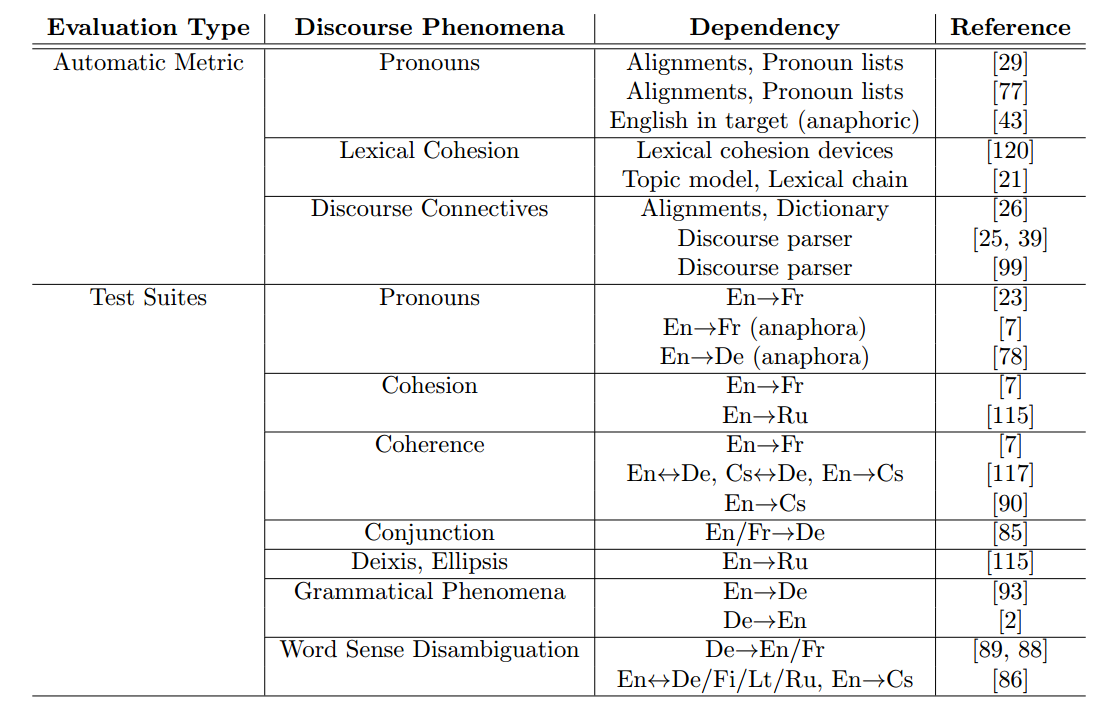
\includegraphics[width=0.7\linewidth]{Images/maruf_2019_discourse_phenomena}
		\caption{Overview of works on discourse phenomena evaluation in MT \cite{maruf_survey_2019}.}
			\label{fig:maruf2019discoursephenomena}
	\end{figure}
		
\end{frame}

\begin{frame}{Evaluation}
	
	
	\begin{itemize}
		\item The evaluation of discourse phenomena in document-level MT, \textit{desiderata}, and particularly the test suites, should:
		\begin{itemize}
			\item Provide inter-sentential context\footnote{in the remainder of this presentation, we refer to inter-sentential context simply as context.};
			\item Focus on context-dependent cases;
			\begin{itemize}
				\item E.g., pronominal anaphora cases in which the antecedent is in a previous sentence (context-dependent), instead of being in the same sentence (context-independent).
			\end{itemize}
			\item Focus on hard cases.
				\begin{itemize}
					\item E.g., when translating English to French, \textbf{he} is easy whereas \textbf{it} is hard to translate because ambiguous.
				\end{itemize}
		\end{itemize} 
	\end{itemize}
	
\end{frame}

\subsection{Automatic metrics}
\begin{frame}{Automatic metrics}

\textbf{Accuracy of Pronoun Translation} \cite{miculicich_werlen_validation_2017}:
	\begin{itemize}
		\item \textit{Compatible languages}: conceived for English to French but it has also been extended to other language pairs.
		\item \textit{Functioning}:
		\begin{itemize}
			\item Align source, reference and candidate translation with GIZA++ plus some heuristics;
			\item Compare candidate and reference pronouns taking into account \textbf{equivalent} pronouns and identical pronouns with \textbf{different forms} (target language-specific);
			\item E.g. \textit{it is difficult} $\rightarrow$ \textit{il/ce/c' est difficile}.
		\end{itemize}
	\end{itemize}

\end{frame}

\begin{frame}{Automatic metrics}
	
\textbf{Pronoun Pair-wise Ranking} \cite{jwalapuram_evaluating_2019}

\begin{itemize}
	\item \textit{Rationale1}: \textbf{ranking-based evaluation} measures can achieve higher correlations with human judgments, as rankings are simpler to obtain from humans and to train models on.
	\item \textit{Compatible languages}: all languages. The metric \textbf{only needs target-side inputs} $\implies$ thus it can be trained and evaluated without the need of a parallel corpus for each source-target pair.
	\item \textit{System input}: a pair $R=(C_r, r)$ and $S=(C_s, s)$ of translations to be compared, where:
	\begin{itemize}
		\item $C_r,C_s$ are the two translations. Each $C$ can comprise one or multiple sentences (context)
		\item $r,s$ are the positions of the pronouns to be compared in the translation $R$ and $S$, respectively.
	\end{itemize} 
\end{itemize}
	
\end{frame}


\begin{frame}{Automatic metrics}
	
\begin{figure}
	\centering
	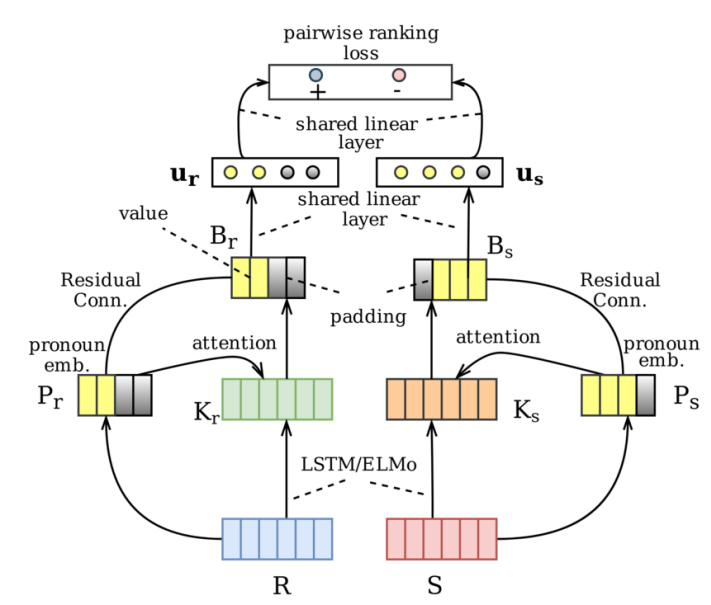
\includegraphics[width=0.55\linewidth]{Images/jwalapuram_2019_pronoun_ranker}
	\caption{Pairwise ranking system by \cite{jwalapuram_evaluating_2019}.}
	\label{fig:jwalapuram2019pronounranker}
\end{figure}

\end{frame}

\begin{frame}{Automatic metrics}
	
	\textbf{Lexical Cohesion extension} \cite{wong_extending_2012}
	
	\begin{itemize}
		\item A \textbf{stemming algorithm} \cite{porter_algorithm_1980} is used to identify word stems for each content word  ; 
		\begin{itemize}
			\item Words with the same stem are defined and counted as \textbf{Repetitions}.
		\end{itemize}
		\item \textbf{WordNet} \cite{fellbaum_semantic_1998} is used to cluster synonims and superordinates into  semantic groups;
		\begin{itemize}
			\item Words belonging to the same semantic group or close semantic groups (near-synonims) are defined and counted as \textbf{Lexical Cohesion Devices} (LCD).
		\end{itemize}
		\item A \textbf{hybrid metric} can then be defined as weighted average of:		
			\begin{itemize}
				\item a \textbf{classic sentence-level metric}, e.g. BLEU, METEOR, TER;
				\item \textbf{a lexical cohesion metric}, e.g. $Repetitions / content\ words$ or $LCD / content\ words$.
			\end{itemize}
		
		
	\end{itemize}
	
\end{frame}



\subsection{Test suites}
\begin{frame}{Test suites}
	
	\begin{itemize}
		\item \cite{bawden_evaluating_2018}: exemplary contrastive test suite, also good model reaching SOTA. Coherence very bad. Need for good models in coherence?
		\item \cite{muller_large-scale_2018}.  Proposal: A Large-Scale Test Set for the Evaluation of Context-Aware Pronoun Translation in Neural Machine Translation.
		\begin{itemize}
			\item Rationale: problems with previous contrastive test suites is that they are either too small to provide stathistical significance \cite{bawden_evaluating_2018} or not adapted to properly test DLNMT systems because lemmatized or not always with context.
			\item similar method will be adopted by \cite{jwalapuram_evaluating_2019}
			\item Focus: inter-sentential anaphora, hard case, , i.e., it → er, sie, es.
		\end{itemize}
	\end{itemize}
	
\end{frame}

\subsection{Remarks and conclusions}
\begin{frame}{Remarks and conclusions}
	
	\begin{itemize}
		\item automatic metrics
		\begin{itemize}
			\item are less expensive than human annotation and thus more easily applicable to all languages 
			\item are noisy because they often rely on other imperfect NLP systems. E.g. alignment and coreference systems.
			\item some automatic metrics might not be enough correlated with human judgment and miss the evaluation of some pronominal functions:
			\begin{itemize}
				\item is the case for APT, for example \cite{guillou_automatic_2018}
			\end{itemize}
			\item there is nothing on coherence although it's the most relevant for post-editors together with cohesion
		\end{itemize}
	
		\item test suites
		\begin{itemize}
			\item systems trained on in-domain data perform better?
		\end{itemize}

		\item what could we do?
		\begin{itemize}
			\item strongly test new automatic metrics against human judgment
			\item semi-automatic metrics: use a high precision automatic metric and a human to evaluate negative cases
			\item keep designing test suites for very restricted scope
		\end{itemize}
	\end{itemize}
	
\end{frame}



		


%\begin{itemize}[noitemsep,topsep=0pt]
%	\item<+(1)-|alert@+(1)> BLUE, METEOR, TER for average quality. Not good enough \cite{maruf_survey_2019}.
%	\item<+(1)-|alert@+(1)> \cite{bawden_evaluating_2018}: exemplary contrastive test suite, also good model reaching SOTA. Coherence very bad. Need for good models in coherence?
%\end{itemize}